\documentclass[12pt]{article}
\usepackage[margin=1in]{geometry}
\usepackage{graphicx}
\graphicspath{ {./} }


\title{Talkatiel Software Requirements and Planning}
\author{Brendan Byers, Ryan Sisco, Iliana J, Aidan Grimshaw}
\date{\today}

\begin{document}
\begin{center}
      \Large\textbf{Talkatiel Software Design Specification and User Interface}\\
      \large\textit{Brendan Byers, Ryan Sisco, Iliana Javier, Aidan Grimshaw, Yufei Zeng}\\
      \large{byersbr, siscor, javieri, grimshaa, zengyu}\\
   \end{center}

\tableofcontents
\pagebreak
\section{User Interface Prototypes}
We have created three user interface prototypes to showcase the key user interactions that will make our app functional.

\begin{center}
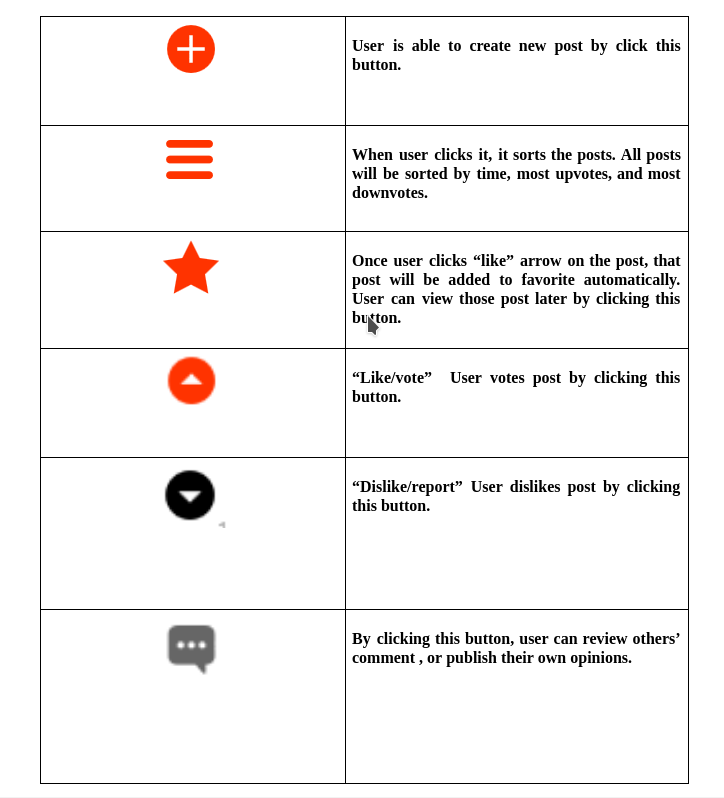
\includegraphics[scale=0.60]{img/ui/uiTable}\linebreak
\textbf{UI Symbol Meanings}
  \end{center}
\pagebreak

\subsection{Creating a New Post}
Users create a new post with a title and text content. When they press the submit button, a new post element is added to the database, with the attributes of title, text content, submission time, upvote/downvote count, and author as specified by the post class diagram.
\begin{center}
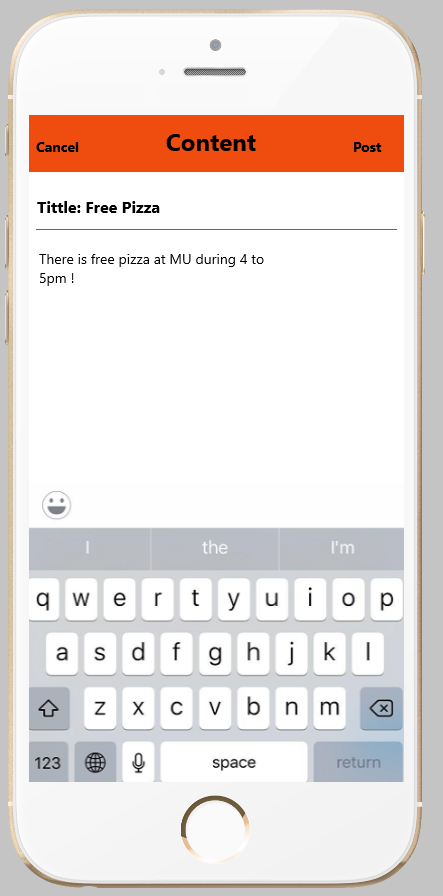
\includegraphics[scale=0.30]{img/ui/post}
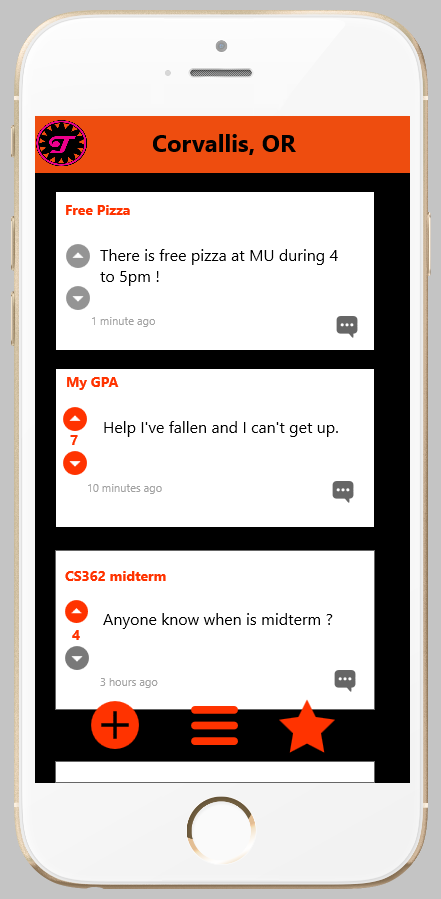
\includegraphics[scale=0.30]{img/ui/post-review}\linebreak
\textbf{Creating a New Post UI}
  \end{center}

\subsection{Auditing New Post}
Post filtering software highlights text that needs to be removed before posting is successful, and prohibits the user from posting until such a condition is met. Examples of prohibited strings include doxxing related strings (phone numbers, addresses), and threat related strings (bomb, kill).
\begin{center}
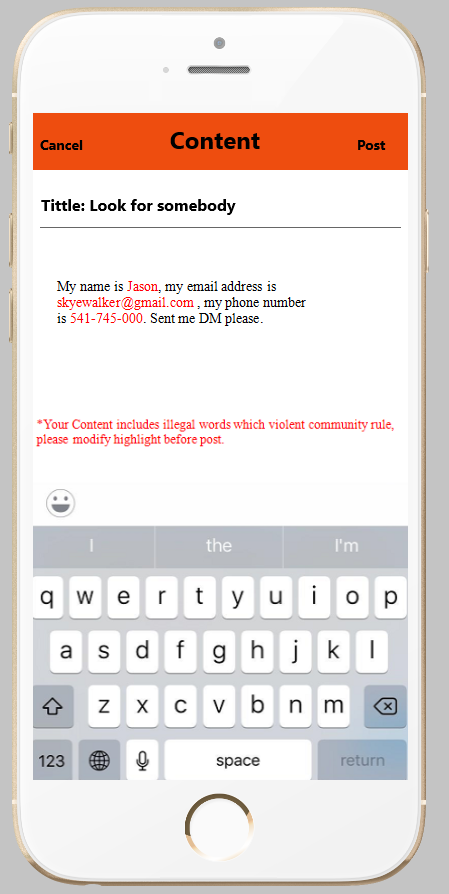
\includegraphics[scale=0.30]{img/ui/bad-post}\linebreak
\textbf{Auditing Result UI}

  \end{center}

\subsection{Viewing Page}
Users view posts on the post viewing page of the app, which is the one that will be loaded when the app starts. Users will view posts sorted by the post sorting function, from which users can select a time range to view posts from, top posts from last 24 hours, week, month, year, or ever. Users will update the posts by pulling down on the top of the app, which will send a request to the server for the updated posts table, which will then be filtered by the post sorting function and displayed to the user in order of time.
\begin{center}
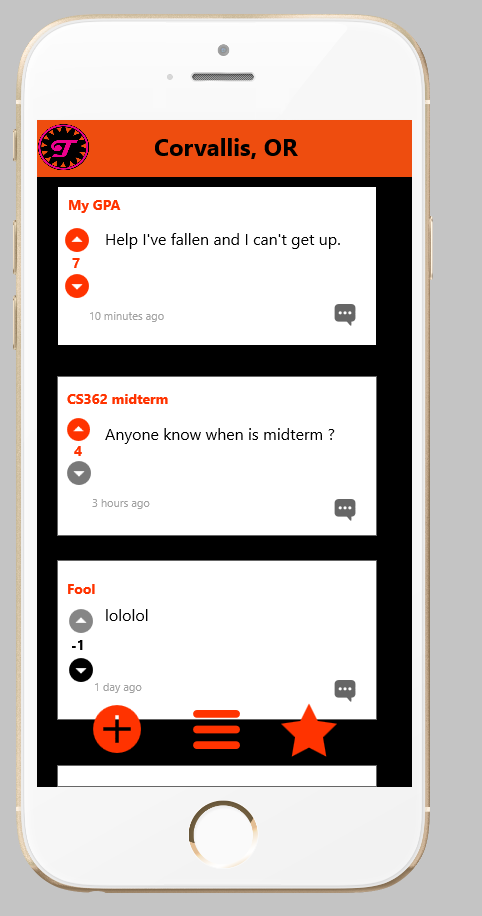
\includegraphics[scale=0.30]{img/ui/view}\linebreak
\textbf{Main Post Page UI}
  \end{center}

\section{Class Diagram}
\begin{center}
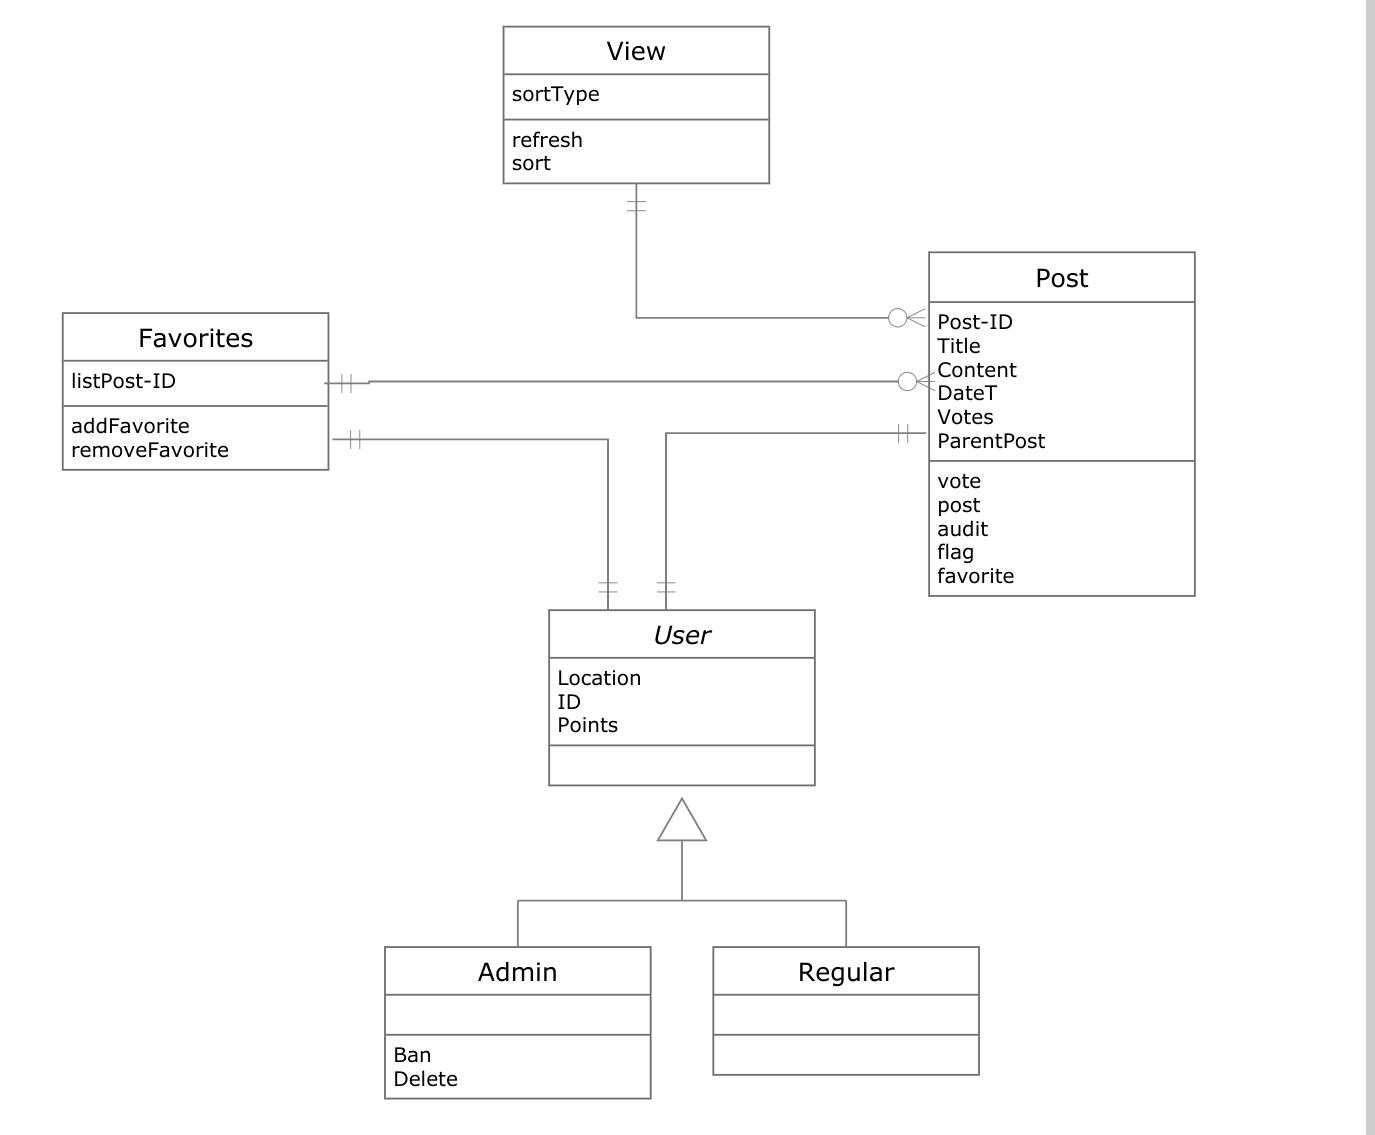
\includegraphics[scale=0.25]{img/uml/ClassDiagram}\linebreak
\textbf{Class Diagram}
  \end{center}

The class diagram consists of four primary classes.  There is the user, view, post and favorites.  The user class is abstract, so a user can either be a regular user or an admin user.  Both types will have location, id and points properties that are tied directly to that user.  The admin has an extra set of functions that allow them to delete a post and ban a user.  Regular users won’t have access to these functions.  The user object will have a single favorites and a single post object tied to it.
The favorites object will store a users favorite posts.  It will hold a list of posts that the users saves in their “favorites” list.  This provides a way for users to view old posts that may be hard to find, allowing them to quickly find them later.  The favorites object will have a list of posts, along with two methods to add and delete posts from the favorites list.  The favorites list will contain 0 or many posts, and the user on the device will only have 1 favorites object.
The post object is the meat of the web app.  Each post object will contain all the information about the post, including post id, title, content, DateTime posted, number of votes, and the id of its parent post.  Along with these parameters it will have a few methods that allow the user to control their posts.  Those methods will allow a user to vote on a post, create a post, audit and verify a post, flag a post for admins, and add the post to a users favorites.  There will be one post object for the user, which they will use to create and favorite posts.  There will be a seperate post object for each post in a users feed.
The post objects in the user feed will be managed by the view object.  This object will manage painting the screen and fetching posts from the server.  It will have a sortType attribute that defines how posts will be shown.  The view object will be able to refresh and sort posts.  There will only be one view object, along with multiple post objects for each post in the feed.
The symbols used in the image above are different than in the lecture notes.  This is because of the software used to create the diagram.  These symbols match those used in database schema and entity-relationship designs.  The double lines mean one and only one.  The circle with the three branching lines means 0 or many, exactly like the 0..* quantifier.

\section{Sequence Diagram}
\subsection{Creating a New Post}
This is the UML for creating a post. It is designed to be quick and simple with minimal computation.

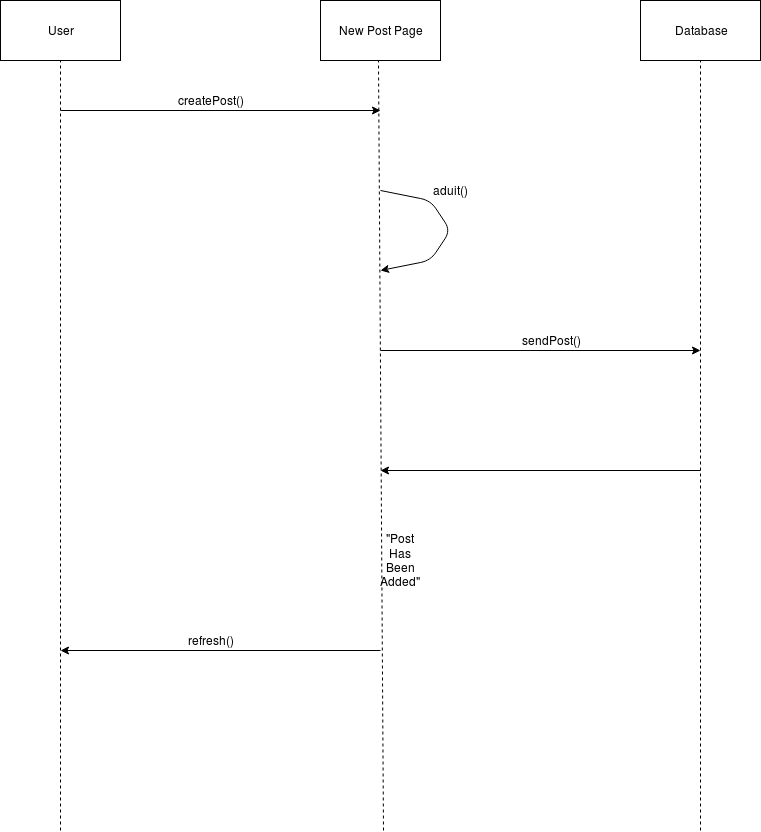
\includegraphics[scale=0.50]{img/uml/createPost}

The user will initiate the new post and be taken to a new post page. They will fill in the requirements. They will hit submit, and their information will be checked to post. If they can post, their submission will be broken from the loop and sent to the database. The information will be updated, the user will be notified, and the page will refresh.
\subsection{Auditing the New Post}
This is the UML for auditing posts. It is made for users to delete their own posts and admins to delete any posts.

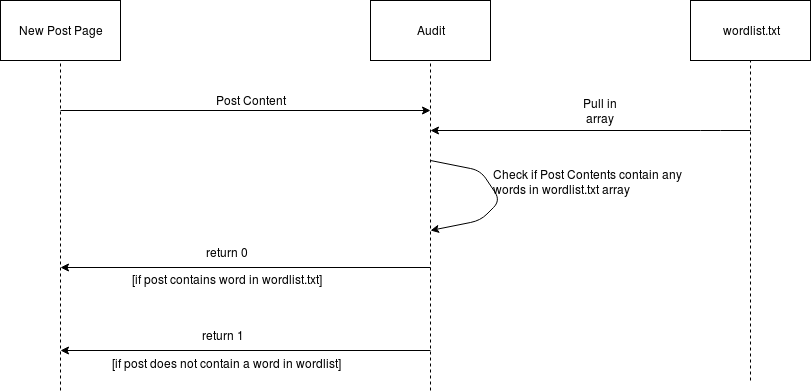
\includegraphics[scale=0.50]{img/uml/audit}

The user will click on a post they want to delete. This will then get checked to see if they are an admin, or if they are the original author. If either condition is met, the post will be deleted from the database. If they fail the if statement, then we know they are a regular user trying to delete someone else’s post.
\subsection{Viewing Post Page}
This its the UML for viewing an entire post. This means that the comments need to be shown. They cannot be upvoted, so the only option a user has is to create a comment.

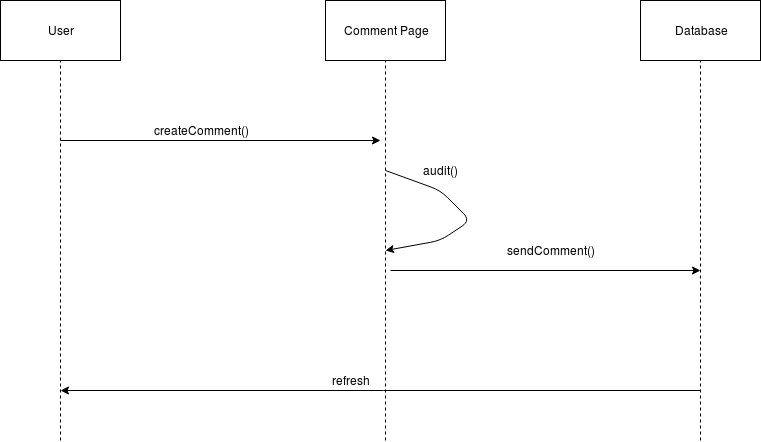
\includegraphics[scale=0.50]{img/uml/createComment}

The user can initiate the comment start, which is taken to the comment page. They will provide the information, and the loop will break once they have met all the conditions. The comment will then be sent to the database, the user will receive a notification, and the page will be refreshed.

\section{Meeting Report}

\subsection{Progress Made This Week}
This week we developed the UML design for the flow of actions that will take place on the app, as well as the UML design of the overall class hierarchy and which functions will belong to which classes. Additionally, we mocked up several use cases that comprise the core of our product.

\subsection{Plans for Next Week}
In the coming week, we plan to continue to develop our ideas and get basic code written for the frontend of the app using HTML, CSS, Javascript, and Bootstrap. Additionally, we will start learning about backend management using Firebase to build a table of users and posts. We will document code both in comments and in external writeups and updated UML designs.

\subsection{Team Member Contributions}
Github Repo Management/Organization- Aidan Grimshaw, Brendan Byers, Ryan Sisco\newline
User Interface Prototype- Yufei Zeng, Aidan Grimshaw\newline
Class Diagrams- Brendan Byers, Iliana Javier\newline
Sequence Diagrams- Ryan Sisco\newline
Meeting Report- Aidan Grimshaw\newline

\end{document}
